% Autogenerated translation of geoChronR-paper.knit.md by Texpad
% To stop this file being overwritten during the typeset process, please move or remove this header

\documentclass[12pt]{book}
\usepackage{graphicx}
\usepackage{fontspec}
\usepackage[utf8]{inputenc}
\usepackage[a4paper,left=.5in,right=.5in,top=.3in,bottom=0.3in]{geometry}
\setlength\parindent{0pt}
\setlength{\parskip}{\baselineskip}
\setmainfont{Helvetica Neue}
\usepackage{hyperref}
\pagestyle{plain}
\begin{document}

\hrule
title: GeoChronR -- an R framework to model and analyze age-uncertain paleogeoscientific timeseries.
journal: "gc"
author:
  - given\emph{name: Nicholas
    surname: McKay
    affiliation: 1
    email: Nicholas.McKay@nau.edu
    corresponding: true
  - given}name: Julien
    surname: Emile-Geay
    affiliation: 2
    email: julieneg@usc.edu
  - given\_name: Deborah
    surname: Khider
    affiliation: 2

\chapter*{If you have more than one corresponding author, add them manually using the following structure:}

\chapter*{Two authors: correspondence\{Daniel Nüst (daniel.nuest@uni-muenster.de) and Josiah Carberry (j.carberry@orcid.org)\}}

\chapter*{Three authors or more: correspondence\{Daniel Nüst (daniel.nuest@uni-muenster.de), Josiah Carberry j.carberry@orcid.org), and Markus Konkol (m.konkol@wwu.de)\}}

\chapter*{If the following line is uncommented, the "corresponding: true" above are ignored}

\chapter*{correspongdingauthors: Daniel Nüst (daniel.nuest@uni-muenster.de) and Josiah Carberry (j.carberry@orcid.org)}

affiliation:
  - code: 1
    address: School of Earth and Sustainability, Northern Arizona University, Flagstaff, AZ 86011
  - code: 2
    address: University of Southern California, Los Angeles, CA
abstract: $\vert$

  Chronological uncertainty is a hallmark of the paleosciences. While many tools have been made available to researchers to produce age models suitable for various settings and assumptions, disparate tools and output formats often discourage integrative approaches. In addition, propagating age model uncertainties to subsequent analyses, and visualizing the results, has received comparatively little attention in the literature and available software. Here we describe GeoChronR, an open-source R package to facilitate these tasks. GeoChronR is built around emerging data standards for the paleosciences (Linked Paleo Data, or LiPD), and offers access to four popular age modeling techniques (Bacon, BChron, Oxcal, BAM). The output of these models is easily stored in LiPD, enabling paleo-aware synchronization, regression, correlation, principal component, and spectral analyses. Five real-world use cases illustrate how to use GeoChronR to facilitate these tasks, and to visualize the results in intuitive ways. 

bibliography: geochronr.bib
running:
  title: The GeoChronR framework
  author: McKay et al.

\chapter*{This section is mandatory even if you declare that no competing interests are present.}

competinginterests: $\vert$
  The authors declare no competing interests.

\chapter*{OPTIONAL:}

algorithms: true

\chapter*{See https://publications.copernicus.org/for\emph{authors/licence}and\_copyright.html, normally used for transferring the copyright, if needed.}

copyrightstatement: $\vert$
  The author's copyright for this publication is transferred to institution/company.

\subsection*{The following commands are for the statements about the availability of data sets and/or software code corresponding to the manuscript.}

\subsection*{It is strongly recommended to make use of these sections in case data sets and/or software code have been part of your research the article is based on.}

availability:
  \#code: $\vert$
  \#  use this to add a statement when having only software code available
  \#data: $\vert$
  \#  use this to add a statement when having only data sets available
  codedata: $\vert$
    use this to add a statement when having data sets and software code available
  \#sample: $\vert$
  \#  use this section when having geoscientific samples available
  \#videosupplement: $\vert$
  \#use this section when having video supplements available
  authorcontribution: $\vert$
    NPM did... JEG did a lot o cheerleading, created lots of bugs, but did manage to write one vignette. DK did...
disclaimer: $\vert$
  disc
acknowledgements: $\vert$
  ack
appendix: $\vert$
  section\{Figures and tables in appendices\}
  Regarding figures and tables in appendices, the following two options are possible depending on your general handling of figures and tables in the manuscript environment:
  subsection\{Option 1\}
  If you sorted all figures and tables into the sections of the text, please also sort the appendix figures and appendix tables into the respective appendix sections.
  They will be correctly named automatically.
  subsection\{Option 2\}
  If you put all figures after the reference list, please insert appendix tables and figures after the normal tables and figures.

  To rename them correctly to A1, A2, etc., please add the following commands in front of them:
  \texttt{\textbackslash{}appendixfigures} needs to be added in front of appendix figures
  \texttt{\textbackslash{}appendixtables} needs to be added in front of appendix tables

  Please add \texttt{\textbackslash{}clearpage} between each table and/or figure. Further guidelines on figures and tables can be found below.
output:
  rticles::copernicus\emph{article: default
  bookdown::pdf}book:

\section*{    base\emph{format: rticles::copernicus}article \# for using bookdown features like @ref()}

introduction

\begin{verbatim}
<!-- Introduction text goes here. -->
\end{verbatim}

\begin{verbatim}
<!-- You can change the name of the section if neccessary using `\introduction[modified heading]`. -->
\end{verbatim}

\begin{verbatim}
<!-- The following settings can or must be configured in the header of this file and are bespoke for Copernicus manuscripts: -->
\end{verbatim}

\begin{verbatim}
<!-- - The `journal` you are submitting to using the official abbreviation. You can use the function `rticles::copernicus_journal_abbreviations(name = '...')` to search the existing journals. -->
\end{verbatim}

\begin{verbatim}
<!-- - Specific sections of the manuscript: -->
\end{verbatim}

\begin{verbatim}
<!--   - `running` with `title` and `author` -->
\end{verbatim}

\begin{verbatim}
<!--   - `competinginterests` -->
\end{verbatim}

\begin{verbatim}
<!--   - `copyrightstatement` (optional) -->
\end{verbatim}

\begin{verbatim}
<!--   - `availability` (strongly recommended if any used), one of `code`, `data`, or `codedata` -->
\end{verbatim}

\begin{verbatim}
<!--   - `authorcontribution` -->
\end{verbatim}

\begin{verbatim}
<!--   - `disclaimer` -->
\end{verbatim}

\begin{verbatim}
<!--   - `acknowledgements` -->
\end{verbatim}

\begin{verbatim}
<!-- See the defaults and examples from the skeleton and the official Copernicus documentation for details. -->
\end{verbatim}

\begin{verbatim}
<!-- **Important**: Always double-check with the official manuscript preparation guidelines at [https://publications.copernicus.org/for_authors/manuscript_preparation.html](https://publications.copernicus.org/for_authors/manuscript_preparation.html), especially the sections "Technical instructions for LaTeX" and "Manuscript composition". -->
\end{verbatim}

\begin{verbatim}
<!-- Please contact Daniel Nüst, `daniel.nuest@uni-muenster.de`, with any problems. -->
\end{verbatim}

\section*{Background}

Quantifying chronological uncertainties, and how they might influence the understanding of past changes is fundamental to the paleogeosciences. 
Without robust error determination, it is impossible to properly assess the extent to which past changes occurred simultaneously across regions or the duration of abrupt events, both of which limit our capacity to apply paleoscientific understanding to modern and future processes.
The need for better infrastructure to both characterize uncertainty, and to explicitly evaluate how age uncertainty impacts the the interpretation of records of past climate, ecology or landscapes, has been long recognized [@Noren2013, (more)]. 
In response to this need, the paleogeoscience community has made substantial advances toward improving geochronological accuracy by:
1. Improving analytical techniques that allow for more precise age determination on smaller and context-specific samples [@Brown\emph{radiocarbon89,@Eglinton96,@Fifield2000,@Eggins2005,@Santos}blank\_2010]
2. Refining our understanding of how past changes in the Earth system impact the age accuracy, for example: improvements to the radiocarbon calibration curve [@Stuiver91,@Stuiver98,intcal references] and advances in our understanding of spatial variability in cosmogenic production rates used in exposure dating [@Balco2009,Masarik2009]
3. Dramatic improvement in the level of sophistication and realism in age-depth models used to estimate the ages of sequences between dated samples [e.g. @Ramsey2009Bayesian, @parnell2008flexible, @Blaauw2010CLAM, @Blaauw2011BACON].

Over the past 20 years, these advances have been widely adopted in the paleogeosciences. 
However, despite the progress made in quantifying uncertainty in ages and in age models, few studies have formally evaluated how chronological uncertainty may have affected their results. 
For instance, whereas the algorithms presented by [@Ramsey2009Bayesian, @parnell2008flexible, @Blaauw2010CLAM, @Blaauw2011BACON] have been broadly used, the overwhelming majority of these studies calculate the single best-estimate model (often a median or mean), use this model to put measured paleoclimatic or paleoenvironmental data on a timescale, and then proceed to analyze the record with little to no reference to the age modeling exercise citep[e.g.][and many others]\{McKay2008,McKay2009\}. 
Typically, any discussions of chronological uncertainties remain qualitative.

This paradigm is beginning to change. 
In recent years a handful of studies have taken advantage of approaches that generate ensembles of age models to evaluate how the results of their analyses and conclusions vary given differences between ensemble members citep\{Haam\emph{Huybers2010,Rhines}JGR2011,Anchukaitis\emph{Tierney2012,Shakun}Nature2012,Marcott\_Science2013, Tierney2013\}. 
By using each ensemble age model to create a time-uncertain ensemble records, and then carrying that ensemble through the analysis, the precise impact of age uncertainty can be formally evaluated. 
This approach, of course, does not address all aspects of uncertainty, but it does offer the broad potential to ascertain which results are robust to chronological uncertainty, and which are not.

Despite its potential to substantially improve uncertainty quantification for the paleogeosciences, this framework is not widely utilized. 
The majority of studies utilizing this approach have been regional [e.g., @Anchukaitis\emph{Tierney2012,@Tierney2013,@mckay}onset\emph{2018, @routson2018\} or global-scale [e.g., @Shakun}Nature2012,@Marcott\_Science2013,@kaufman2020HoloceneGMST] syntheses.
Occasionally, primary publications of new records incorporate time-unceratin analysis into their studies [@Boldt2015,more], but this remains rare. 
We suggest that there are several reasons for the lack of adoption of these techniques:

\begin{enumerate}
\item For synthesis studies, the necessary geochronological data are not publicly available for the vast majority of records. Even when they are available, the data are archived in diverse and unstructured data formats. Together, this makes what should be a simple process of aggregating and preparing data for analysis prohibitively time-consuming;
\item For studies of new and individual records, few tools for ensemble analysis are available, and those that are require a degree of comfort with coding languages and scientific programming that is rare among paleogeoscientists;
\item There is a disconnect between age-model development and time-uncertain analysis. Published approaches have utilized either simplified age-modeling approaches [@Haam\emph{Huybers2010], or specialized approaches not used elsewhere in the community [@Shakun}Nature2012,@Anchukaitis\emph{Tierney2012,@Marcott}Science2013,@Tierney2013,@Routson2018]. 
Extracting the relevant data from commonly-used age-modelling algorithms, creating time-uncertain ensembles, then reformatting those data for analysis in available tools typically requires the development of extensive custom codesets. 
\end{enumerate}

\section*{Motivation}

GeoChronR is built to lower the barriers to broader adoption of these emerging methods.
It provides an easily-accessibly, open-source and extenisble software package of industry-standard and cutting-edge tools that provides users a single environment to create, analyse, and visualize time-uncertain data.
GeoChronR is designed around emerging standards in the paleogeosciences that connects users to growing libraries of standardized datasets formatted in the Linked PaleoData format [@LiPD] and [@neotoma].

\section*{Outline of manuscript}

This manuscript describes the design, analytical underpinnings and most common use cases of GeoChronR.
Section @ref(\#age-modeling) describes the integration of age modelling algorithms with GeoChronR.
Section @ref(\#age-uncertain-analysis) details the methods implemented for age uncertain analysis, and section @ref(\#use-cases) provides five real-world examples of how GeoChronR can be used for scientific workflows.

\begin{verbatim}
<!-- Age modeling section -->
\end{verbatim}

\chapter*{Age Modeling with GeoChronR \{\#age-modeling\}}

Context: \href{https://doi.org/10.1177/0959683616675939}{Trachsel \& Telford}

\section*{Bacon}

\section*{BChron}

\section*{Oxcal}

\section*{Banded Age Model (BAM)}

\begin{verbatim}
<!-- Analysis section -->
\end{verbatim}

\chapter*{Age-uncertain data analysis in GeoChronR \{\#age-uncertain-analysis\}}

Intro on analytical approach, using ensembles....

\section*{Correlation}

\section*{Regression}

\section*{Principal Component Analysis}

\section*{Spectral Analysis}

\begin{verbatim}
<!-- Viz section -->
\end{verbatim}

\chapter*{Visualization with GeoChronR}

ggplot philosophy. Customization. 

\subsection*{Timeseries}

\subsection*{Geospatial}

WTF does geospatial mean anyway? 
NM: It means mapping.

\subsection*{Spectral Analysis}

\chapter*{Use cases \{\#use-cases\}}

We now illustrate the use of these tools on four use cases. The first example shows how to create age ensembles on different archives, and how to visualize the timing of abrupt events with appropriate uncertainty quantification. The second example shows how to quantify similarities in age-uncertain records. The third introduces the topic of age-uncertain calibrations, the fourth quantifies multivariate relationships using principal components analyses, and the fifth deal with spectral analysis. 

\section*{Creating an age ensemble}

A common first task when using geoChronR is to create an age ensemble, either because the user is developing a new record, or because the age ensemble data for the record they are interested is unavailable.
As described in section X.Y workflows for four published age quantification programs are integrated into geoChronR.
Bacon [@bacon], BChron [@parnell2008flexible], and OxCal [@ramsey2008deposition] are Bayesian age-deposition models that estimate posteriors on age-depth relationships with different assumptions and methodologies.
BAM [@BAM] was designed to probabilistically simulate counting uncertainty in banded archives, such as corals, ice cores, or varved sediments, but can also be used to simulate age uncertainty for any record, and is useful when the data or metadata required to calculate an age-depth model are unavailable.
All four methods are mostly simply used in geoChronR with a LiPD file that contains the chronological measurements, and the functions \texttt{runBacon(L)}, \texttt{runBchron(L)}, \texttt{runOxcal(L)} and \texttt{runBam(L)}.
These functions take LiPD objects as inputs, and return updated LiPD objects that include age-ensemble data generated by the respective software packages.
Typically, additional parameters are needed for to optimally run the algorithms.
When these parameters are not included, geoChronR will run in interactive mode, asking the user which variables and parameters they would like to model.
These parameter choices are printed to the screen during while the program runs, or are available later with the function \texttt{getLastVarString()}.
By specifying these parameters, age model creation can be scripted and will run in non-interactive mode.
In this use case, we'll use geoChronR and BChron [@parnell2008flexible] to calculate an age ensemble for the Hulu Cave \$delta\textasciicircum{}\{18\}\$O speleothem record [@hulu2001], and BAM [@BAM] to simulate age uncertainties for the GISP2 ice core \$delta\textasciicircum{}\{18\}\$O dataset [@alley].
The \texttt{plotChronEns(hulu)} function will plot an age-depth model and uncertainties derived from the age ensemble.

```

\section*{[1] "Found it! Moving on..."}

\section*{[1] "Found it! Moving on..."}

\section*{[1] "plotting your chron ensemble. This make take a few seconds..."}

```

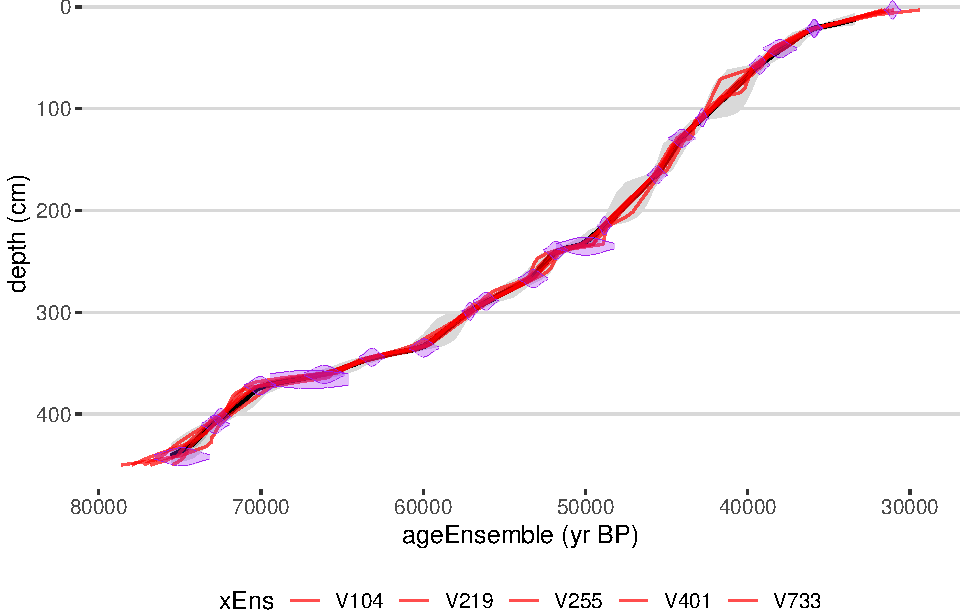
\includegraphics{geoChronR-paper_files/figure-latex/unnamed-chunk-3-1.pdf}$<$!-- --$>$ 
After an age ensemble has been added to a LiPD object, the user can visualize the ensemble timeseries using \texttt{plotTimeseriesEnsRibbons()} and \texttt{plotTimeseriesEnsLines()}.
GISP2 \$delta\textasciicircum{}\{18\}\$O is plotted with age uncertainty, using both functions, in figure x.

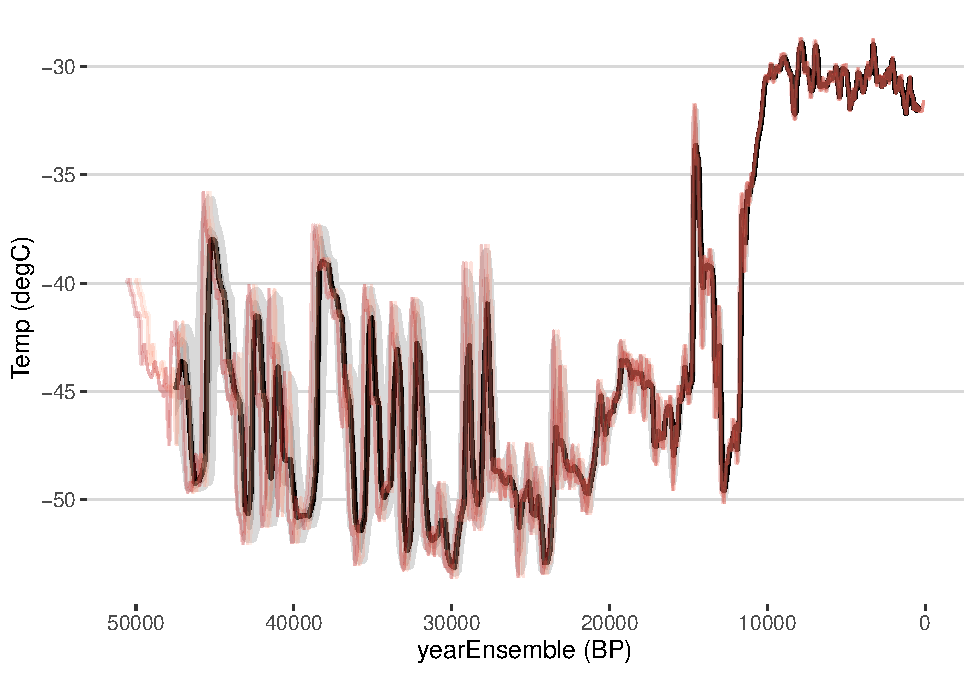
\includegraphics{geoChronR-paper_files/figure-latex/unnamed-chunk-5-1.pdf}$<$!-- --$>$ 

\section*{Correlation}

Now that the user has generated age ensembles for the two datasets, they're interested to see if a correlation between the two datasets is robust to the age uncertainty modeled here.
On multi-millennial timescales, the two datasets have similarities, and previous work has suggested that could events during the Last Glacial period, which are observed in the GISP2 record, can impact the Asian Monsoon and be observed is speleothem records such as the Hulu Cave dataset. (NM: add references here and flesh out background)
The \texttt{corEns()} function in geoChronR will calculate ensemble correlations across age-uncertain datasets, such as these.
\texttt{corEns()} will also sample across ensembles in the paleoData as well, if present.
Here we calculate correlations during the period of overlap in 500 yr steps, determining significance for each pair of ensemble members while accounting for autocorrelation.

The results show consistently negative correlations, although 15.21\% of the ensemble members are positive.
However, only 0.91\% are significant after accounting for serial autocorrelation.

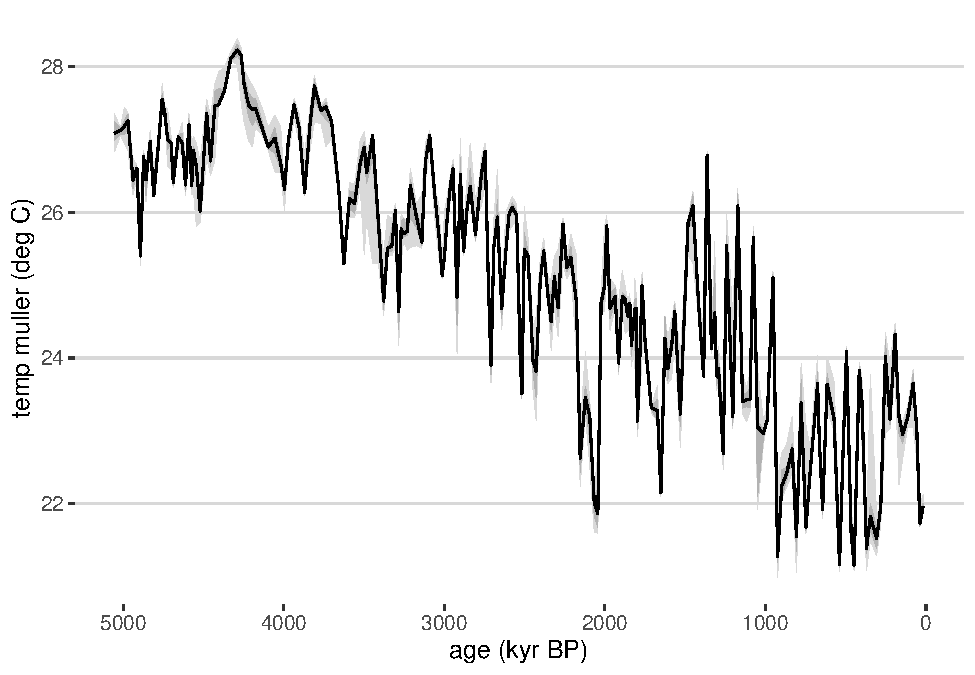
\includegraphics{geoChronR-paper_files/figure-latex/unnamed-chunk-7-1.pdf}$<$!-- --$>$ 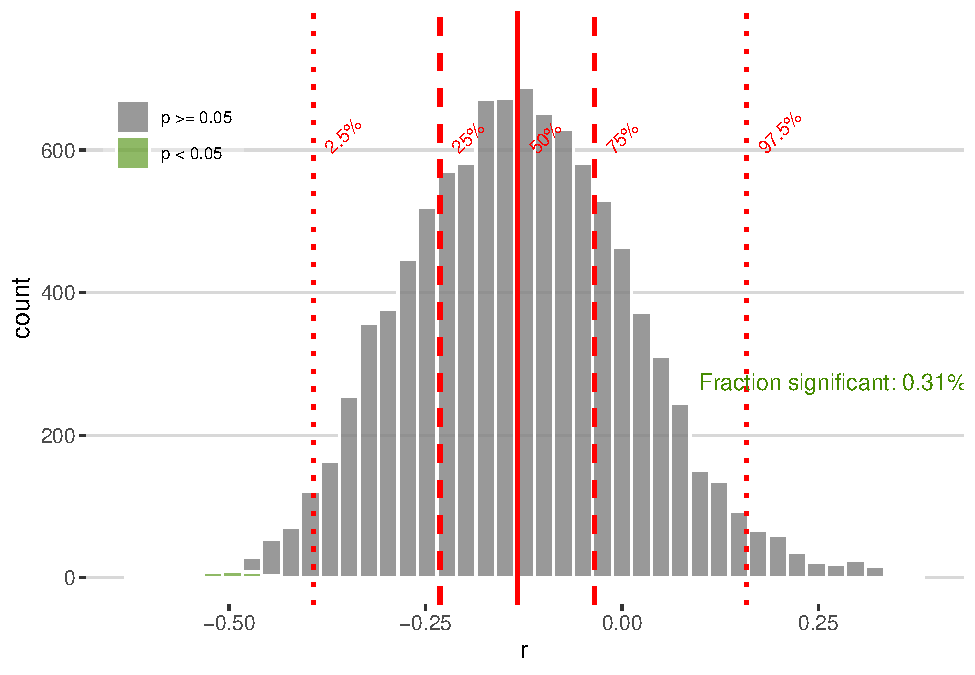
\includegraphics{geoChronR-paper_files/figure-latex/unnamed-chunk-7-2.pdf}$<$!-- --$>$ 

In this use case, we demonstrate how a user could calculate and visualize and age-uncertain correlation between the Hulu speleothem \$delta\textasciicircum{}\{18\}mathrm\{O\}\$ record and the GISP2 ice core \$delta\textasciicircum{}\{18\}mathrm\{O\}\$ record. (Introduction about why a user might want to do an age uncertain correlation between Hulu and GISP2).

\section*{Age-uncertain Calibration}

A natural extension of ensemble correlation is ensemble regression.
Although there are use cases where regressing one age-uncertain variable onto another is called for, here we regress an age-uncertain paleoclimate proxy onto time-certain instrumental to develop a calibration-in-time.
For this use case, we reproduce the results of @Boldt:2015, where the authors calibrate a spectral reflectance measure of chlorophyll abundance to temperature in Northern Alaska.

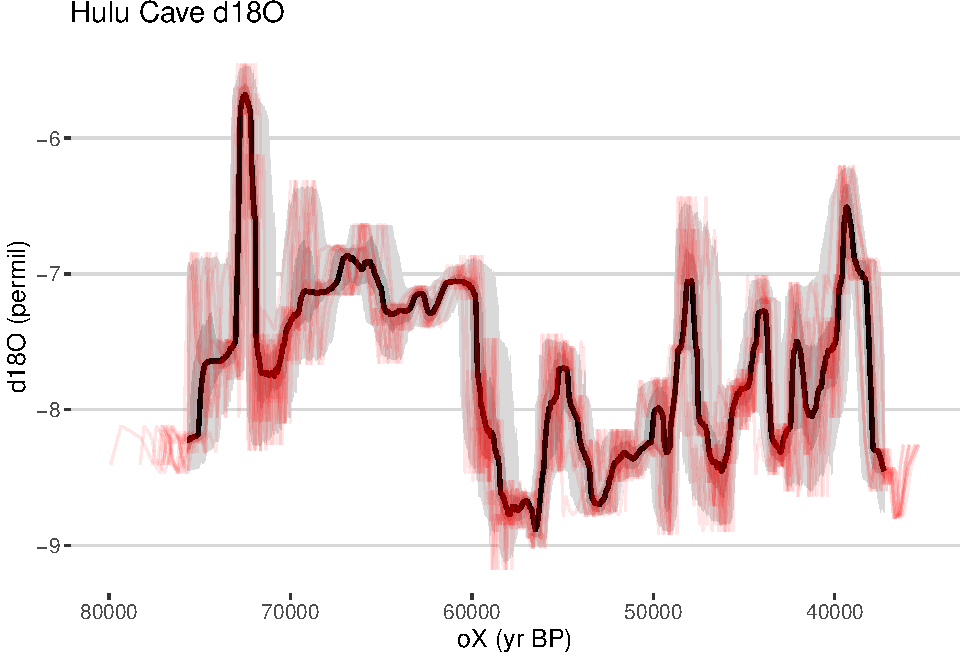
\includegraphics{geoChronR-paper_files/figure-latex/unnamed-chunk-9-1.pdf}$<$!-- --$>$ 
Figure captions.

\section*{Principle Component Analysis}

Thus far, the use cases have highlighted age-uncertain analyses of one or two sites, however quantifying the effects of age uncertainty can be even more impactful over large spatial datasets. 
Here we showcase how to use geoChronR to perform age-uncertain principle components analysis (PCA), also known as Monte Carlo Empirical Orthogonal Function (MCEOF) analysis, pioneered by @anchukaitis2013mceof.
In this example, we examine the Arctic 2k database [@McKayKaufman2014McKayKaufman2014].

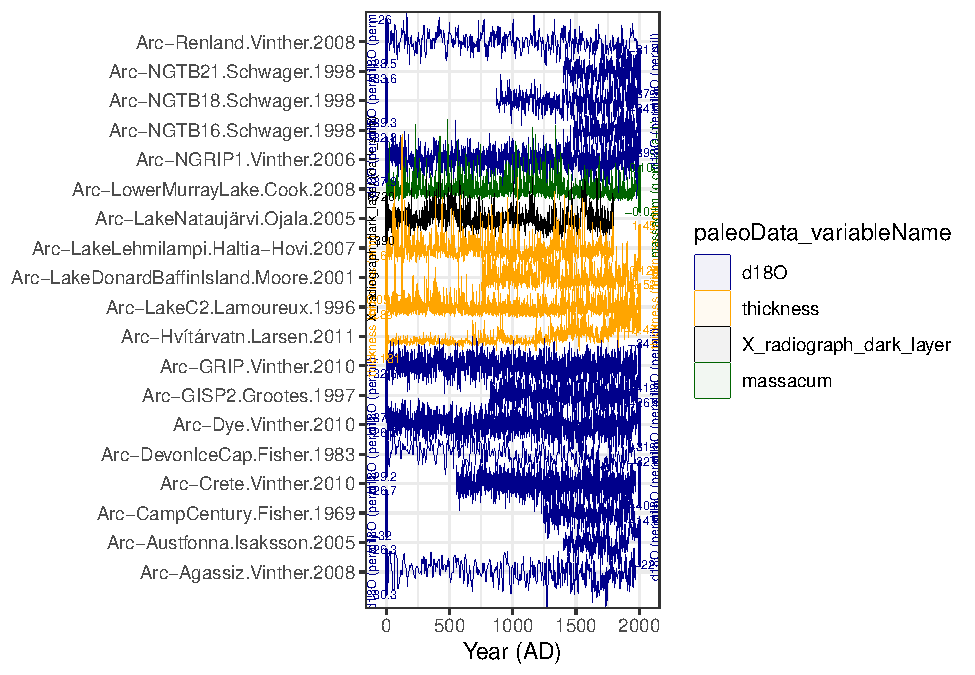
\includegraphics{geoChronR-paper_files/figure-latex/unnamed-chunk-11-1.pdf}$<$!-- --$>$ 

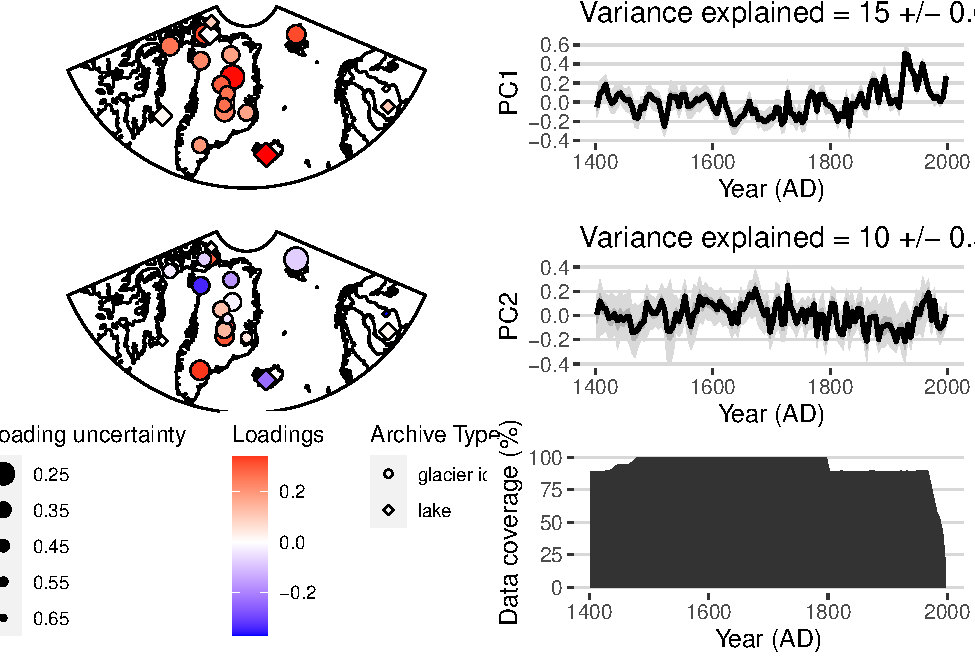
\includegraphics{geoChronR-paper_files/figure-latex/unnamed-chunk-13-1.pdf}$<$!-- --$>$ 

\section*{Spectral Analysis}

\chapter*{Discussion \& Conclusion}

\begin{itemize}
\item Strengths, weaknesses and shortcomings of our approach
\item Next steps; where does age-uncertain work go from here?
\item GeoChronR plans, longevity, etc
\end{itemize}

\chapter*{Everything below are useful examples of how to use RMarkdown}

Subsection text here.

\subsection*{Subsubsection Heading Here}

Subsubsection text here.

\chapter*{Content section with citations}

See the \href{http://rmarkdown.rstudio.com/authoring_bibliographies_and_citations.html}{R Markdown docs for bibliographies and citations}.

Copernicus supports biblatex. I put the .bib entries from the Paleocube proposal into \texttt{geochronr.bib}. Citations work like this:

Read [@Evans\_QSR13], and [see @PRYSM].

\chapter*{Content section with R code chunks}

You should always use \texttt{echo = FALSE} on R Markdown code blocks as they add formatting and styling not desired by Copernicus.
The hidden workflow results in 42.

You can add verbatim code snippets without extra styles by using \texttt{}`\texttt{} without additional instructions.

\texttt{
sum $<$- 1 + 41
}

\chapter*{Content section with list}

If you want to insert a list, you must

\begin{itemize}
\item leave
\item empty lines
\item between each list item
\end{itemize}

```
- leave

\begin{itemize}
\item empty lines
\item between each list item
```
\end{itemize}

\chapter*{Examples from the official template}

\section*{FIGURES}

When figures and tables are placed at the end of the MS (article in one-column style), please add clearpage between bibliography and first table and/or figure as well as between each table and/or figure.

\subsection*{ONE-COLUMN FIGURES}

Include a 12cm width figure of Nikolaus Copernicus from \href{https://en.wikipedia.org/wiki/File:Nikolaus_Kopernikus.jpg}{Wikipedia} with caption using R Markdown.

begin\{figure\}
includegraphics[width=8.3cm]\{Nikolaus\_Kopernikus\} caption\{one column figure\}label\{fig:unnamed-chunk-15\}
end\{figure\}

\subsection*{TWO-COLUMN FIGURES}

You can also include a larger figure.

begin\{figure\}
includegraphics[width=12cm]\{Nikolaus\_Kopernikus\} caption\{two column figure\}label\{fig:unnamed-chunk-16\}
end\{figure\}

\section*{TABLES}

You can ad LaTeX table in an R Markdown document to meet the template requirements.

\subsection*{ONE-COLUMN TABLE}

begin\{table\}[t]
caption\{TEXT\}
begin\{tabular\}\{l c r\}
tophline

a \& b \& c \textbackslash{}
middlehline
1 \& 2 \& 3 \textbackslash{}

bottomhline
end\{tabular\}
belowtable\{Table Footnotes\}
end\{table\}

\subsection*{TWO-COLUMN TABLE}

begin\{table*\}[t]
caption\{TEXT\}
begin\{tabular\}\{l c r\}
tophline

a \& b \& c \textbackslash{}
middlehline
1 \& 2 \& 3 \textbackslash{}

bottomhline
end\{tabular\}
belowtable\{Table footnotes\}
end\{table*\}

\section*{MATHEMATICAL EXPRESSIONS}

All papers typeset by Copernicus Publications follow the math typesetting regulations given by the IUPAC Green Book (IUPAC: Quantities, Units and Symbols in Physical Chemistry, 2nd Edn., Blackwell Science, available at: http://old.iupac.org/publications/books/gbook/green\emph{book}2ed.pdf, 1993).

Physical quantities/variables are typeset in italic font (t for time, T for Temperature)

Indices which are not defined are typeset in italic font (x, y, z, a, b, c)

Items/objects which are defined are typeset in roman font (Car A, Car B)

Descriptions/specifications which are defined by itself are typeset in roman font (abs, rel, ref, tot, net, ice)

Abbreviations from 2 letters are typeset in roman font (RH, LAI)

Vectors are identified in bold italic font using vec\{x\}

Matrices are identified in bold roman font

Multiplication signs are typeset using the LaTeX commands \texttt{\textbackslash{}times} (for vector products, grids, and exponential notations) or \texttt{\textbackslash{}cdot}

The character * should not be applied as mutliplication sign

\section*{EQUATIONS}

\subsection*{Single-row equation}

Unnumbered equations (i.e. using \texttt{\$\$} and getting inline preview in RStudio) are not supported by Copernicus.

begin\{equation\}
1 times 1 cdot 1 = 42
end\{equation\}

begin\{equation\}
A = pi r\textasciicircum{}2
end\{equation\}

begin\{equation\}
x=frac\{2bpmsqrt\{b\textasciicircum{}\{2\}-4ac\}\}\{2c\}. \\end\{equation\}

\subsection*{Multiline equation}

begin\{align\}
\& 3 + 5 = 8\textbackslash{}
\& 3 + 5 = 8\textbackslash{}
\& 3 + 5 = 8
end\{align\}

\section*{MATRICES}

\$\$
begin\{matrix\}
x \& y \& z\textbackslash{}
x \& y \& z\textbackslash{}
x \& y \& z\textbackslash{}
end\{matrix\}
\$\$

\section*{ALGORITHM}

If you want to use algorithms, you can either enable the required packages in the header (the default, see \texttt{algorithms: true}), or make sure yourself that the LaTeX packages \texttt{algorithms} and \texttt{algorithmicx} are installed so that \texttt{algorithm.sty} respectively \texttt{algorithmic.sty} can be loaded by the Copernicus template.
Copernicus staff will remove all undesirable packages from your LaTeX source code, so please stick to using the header option, which only adds the two acceptable packages.

begin\{algorithm\}
caption\{Algorithm Caption\}
label\{a1\}
begin\{algorithmic\}
STATE \$igets 10\$
IF \{\$igeq 5\$\}
        STATE \$igets i-1\$
ELSE
        IF \{\$ileq 3\$\}
                STATE \$igets i+2\$
        ENDIF
ENDIF
end\{algorithmic\}
end\{algorithm\}

\section*{CHEMICAL FORMULAS AND REACTIONS}

For formulas embedded in the text, please use \texttt{\textbackslash{}chem\{\}}, e.g. chem\{A rightarrow B\}.

The reaction environment creates labels including the letter R, i.e. (R1), (R2), etc.

\begin{itemize}
\item \texttt{\textbackslash{}rightarrow} should be used for normal (one-way) chemical reactions
\item \texttt{\textbackslash{}rightleftharpoons} should be used for equilibria
\item \texttt{\textbackslash{}leftrightarrow} should be used for resonance structures
\end{itemize}

begin\{reaction\}
A rightarrow B \textbackslash{}
end\{reaction\}
begin\{reaction\}
Coper rightleftharpoons nicus \textbackslash{}
end\{reaction\}
begin\{reaction\}
Publi leftrightarrow cations
end\{reaction\}

\section*{PHYSICAL UNITS}

Please use \texttt{\textbackslash{}unit\{\}} (allows to save the math/\texttt{\$} environment) and apply the exponential notation, for example ( 3.14,unit\{km,h\textasciicircum{}\{-1\}\} ) (using LaTeX mode: \texttt{\textbackslash{}( 3.14\textbackslash{},\textbackslash{}unit\{...\} \textbackslash{})}) or unit\{0.872,m,s\textasciicircum{}\{-1\}\} (using only \texttt{\textbackslash{}unit\{0.872\textbackslash{},m\textbackslash{},s\textasciicircum{}\{-1\}\}}).

conclusions

The conclusion goes here.
You can modify the section name with  \texttt{\textbackslash{}conclusions[modified heading if necessary]}.

\end{document}
